\documentclass{beamer}
\usetheme{default}
\setbeamertemplate{navigation symbols}{}
%	
\usepackage{subfig}
\usepackage{amsmath, amsthm, amssymb}
\usepackage{float}
\usepackage{rotating}
\usepackage{graphicx}
\usepackage{longtable}
\usepackage{xcolor}
\usepackage{bm}
\usepackage{tikz}
\usetikzlibrary{shapes}
\tikzset{My Arrow Style/.style={single arrow, fill=red!50, anchor=base, align=center,text width=.5cm,rotate =270}}
\newcommand{\MyArrow}[2][]{\tikz[baseline] \node [My Arrow Style,#1] {#2};}
\tikzset{My 2Arrow Style/.style={single arrow, fill=red!50, anchor=base, align=center,text width=.5cm,rotate =90}}
\newcommand{\MyArrowUp}[2][]{\tikz[baseline] \node [My 2Arrow Style,#1] {#2};}
\newcommand{\bmat}{\begin{matrix}}
\newcommand{\emat}{\end{matrix}}
\newcommand{\EE}{\mathbb E}

\newtheorem{acknowledgement}[theorem]{Acknowledgement}
\newtheorem{algorithm}[theorem]{Algorithm}
\newtheorem{assumption}{Assumption}
\newtheorem{axiom}{Axiom}
\newtheorem{case}[theorem]{Case}
\newtheorem{claim}[theorem]{Claim}
\newtheorem{conclusion}[theorem]{Conclusion}
\newtheorem{condition}[theorem]{Condition}
\newtheorem{conjecture}{Conjecture}
\newtheorem{criterion}[theorem]{Criterion}
\newtheorem{proposition}{Proposition}
\newtheorem{summary}[theorem]{Summary}
\newtheorem{exercise}{Exercise}
\newtheorem{notation}{Notation}
\newtheorem{remark}{Remark}
%\graphicspath{{graphs//}}

\title { Optimal Fiscal
policies in some economies with incomplete asset markets}
\author{Anmol Bhandari, David Evans, Mikhail Golosov, Thomas J. Sargent}

\date{September 2013}
% \today will show current date.
% Alternatively, you can specify a date.
%
\begin{document}
%
\begin{frame}
\titlepage

\end{frame}
\section{Introduction}
\subsection{}
\begin{frame}
\frametitle{What do we do?}
We study optimal taxation under commitment with
\begin{itemize}
 \item \textbf{Representative agent}

 \item \textbf{Incomplete markets}

 \quad \color{red}$\rightarrow$ \color{black} assets with more general payoff structures

 \item \textbf{Linear tax schedules}

 \quad \color{red}$\rightarrow$ \color{black}Government levies a proportional tax on labor earnings 

 \item \textbf{Aggregate shocks}

 \quad \color{red}$\rightarrow$ \color{black} To productivities, government expenditure etc.

 \end{itemize}
\end{frame}


\begin{frame}
\frametitle{What are we after?}

\begin{enumerate}
\item Existing literature studies two extremes : economies with comple markets (LS) and economies with risk free bonds (AMSS)
\item We trace out intermediate cases where the asset traded provides partial spanning
 \item In particular study how the payoff structure affect long run properties of optimal government policies and equilibrium allocations?
\end{enumerate}

\end{frame}


\section{Environment}
\subsection{}

\begin{frame}
 \frametitle{Environment}
 \begin{itemize}
 \item \textbf{Uncertainty}: Markov aggregate shocks $s_t$
  \item \textbf{Demography}: infinitely lived representative agent plus a benevolent planner
  \item \textbf{Technology}: Output  $\theta_{t} l_{t}$ is linear in labor supply
  \item \textbf{Preferences }(Households)
  \begin{equation*}
\mathbb{E}_{0}\sum_{t=0}^{\infty } \beta^t  U\left(
c(s^t),l(s^t)\right)  \label{utility lifetime}
\end{equation*}%
 \end{itemize}

\end{frame}

\begin{frame}
 \frametitle{Environment, II}
 \begin{itemize}
\item \textbf{Asset markets}: Private sector has complete markets; Government trades are retricted
  \item \textbf{Linear Taxes}: Agent $i$'s tax bill
\[- T_t + \tau_t \theta_{t}l_{t}\]

\item[]
  \item \textbf{Budget constraints}
  \begin{itemize}
   \item Agents: $ c_{t}+b_{t}=\left( 1-\tau _{t}\right) \theta _{t}l_{t}+R_{t-1}b_{t-1}+T_{t}$
\item Government: $g_{t}+B_{t}+T_t=\tau _{t}\theta_{t}l_{t}+R_{t-1}B_{t-1}$
  \end{itemize}

\item[]
  \item \textbf{Market Clearing}
  \begin{itemize}
   \item Goods: $c_{t}+g_t = \theta _{t} l_{t}$

   \item Assets: $b_{t}+B_{t}=0$
\end{itemize}
  \item[]

\item \textbf{Initial conditions}: Distribution of assets $b_{-1}$ and $B_{-1}$
\end{itemize}

\end{frame}


\begin{frame}
 \frametitle{Ramsey Problem}

\begin{definition}
\textbf{Allocation, price system, government policy}: Standard

\end{definition}

\begin{definition}
\textbf{Competitive equilibrium}: Given $\left(b_{-1},B_{-1}\right) $ and $\left\{ \tau _{t},T_{t}\right\} _{t=0}^{\infty }$
all allocations are chosen optimally, markets clear \footnote{Usually, we impose only  ``natural'' debt limits. }
\end{definition}

\begin{definition}
\textbf{Optimal competitive equilibrium}: A welfare-maximizing competitive
equilibrium for a given $\left( b_{-1},B_{-1}\right) $
\end{definition}

 \end{frame}
 
 
 \begin{frame}
 \frametitle{Sequential problem}  
\[
	\max_{\{c_t,l_t,b_t\}} \EE_0\sum_{t=0}^\infty \beta^t U(c_t,l_t)
\]subject to
\begin{align*}
	\frac{b_{t-1}U_{c,t-1}}{\beta} = \frac{\EE_{t-1} p_t U_{c,t}}{p_t U_{c,t}}\EE_t\sum_{j=0}^\infty\beta^j\left( U_{c,t+j}c_{t+j}+U_{l,t+j}l_{t+j}\right)\text{  for $t\geq 1$ }\\
	b_{-1} = \frac1{U_{c,0}}\EE_0\sum_{t=0}^\infty \beta^t\left(U_{c,t}c_t+U_{l,t}l_t\right)\\
	c_t + g_t = \theta_t l_t
\end{align*}
Where $p_t$ is an iid random variable, representing an exogenous restriction on payoff structure of government assets.  Note that this sequential problem is restricting $T_t = 0$ for all $t$.  This is necessary for our analytical results.  We will show later, numerically, that this assumption is not restrictive.
  \end{frame}
  
 \begin{frame}
\frametitle{Optimal payoff structures}
\begin{itemize}
\item The planner's problem with state contingent debt can be represented as the problem above without the $t\geq1$ measurability restrictions.
\item  It can be thought of then as the planner choosing a payoff structure $p_t$, such that the measurability constraints for $t\geq 1$ are always satisfied.
\item  The optimal allocation then defines the optimal payoff structure chosen to be
\[
	p_t = \frac{\beta}{U_{c,t}b_{t-1}}\EE_t\sum_{j=0}^\infty\beta^j\left(U_{c,t+j}c_{t+j}+U_{l,t+j}l_{t+j}\right)
\]where
\[
	b_{t-1} = \frac{\beta}{U_{c,t-1}}\EE_{t-1}\sum_{j=0}^\infty\beta^j\left(U_{c,t+j}c_{t+j}+U_{l,t+j}l_{t+j}\right)
\]under the normalization $\frac{\EE_{t-1} p_t U_{c,t}}{U_{c,t-1}} = 1$
\end{itemize}
\end{frame} 

\section{Quasilinear}
\subsection{}
 
\begin{frame}
	\frametitle{Quasilinear FOC}
	The familiar first order conditions for the planner's problem where preferences are given by $U(c,l) = c - \frac{l^{1+\gamma}}{1+\gamma}$ are
	\begin{align*}
		1 = \mu +\xi_t\\
		-l_t^\gamma+\mu(1+\gamma)l_t^\gamma+\theta_t\xi_t = 0
	\end{align*}Where $\mu$ is the Lagrange multiplier on the implimentability constraint and $\beta^t\xi_t$ is the multiplier of the resource constraint.   These equations give the tax rate $\tau$ as a function of $\mu$
	\[
		\tau(\mu) = \frac{\gamma\mu}{(1+\gamma)\mu-1}
	\] and the period government surplus 
	\[
		S_t(\tau) = \theta_t^\frac\gamma{1+\gamma}(1+\tau)^\frac1\gamma\tau-g_t
	\]
\end{frame}

\begin{frame}
	\frametitle{Quasilinear Asset Structure}
	Under the i.i.d. assumption, the optimal payoff structure chosen by the planner is given by the equation
	\[
		p = (1-\beta)\frac{St(\tau)}{\EE S(\tau)} + \beta
	\]where $\tau$ is the optimal tax rate given government debt $b$. 
	\begin{lemma}  Let $p_{\theta,g}(b)$ be the payoff chosen by the planner in aggregate state $(\theta,g)$ when government debt is given by $b$.  Then $p_{\theta,g}(b)$ will, generically, be a one-to-one function of $b$.  If $g\EE\theta^\frac{\gamma}{1+\gamma}-\theta^\frac{\gamma}{1+\gamma}\EE g > (<) 0$ then $p_{\theta,g}(b)$ will be an increasing (decreasing) function of $b$. 
	\end{lemma}
\end{frame}

  \begin{frame}
   \frametitle{Graphs }
    a graph that explains the main parts of the theorem
   
   - payoff structures and taxes as a function of initial debt
  \end{frame}

  
  
\begin{frame}
 	\frametitle{Incomplete Markets Solution}
	With quasilinear preferences the measurability constraints for the incomplete markets problem can be written as the period by period constraint
	\[
		\frac{p_t b_{t-1}}\beta = c_t - l_t^{1+\gamma} + b_t 
	\]under the normalization of $\EE_{t-1} p_t = 1$  The first order conditions associated with this problem are
	\begin{align*}
		1 = \mu_t + \xi_t\\
		-l_t^\gamma+\mu_t(1+\gamma)l_t^\gamma+\theta_t\xi_t = 0\\
		\mu_t = \EE_t p_{t+1}\mu_{t+1}
	\end{align*}  Where $\beta^t\mu_t$ is the multiplier on the period by period budget constraint and $\beta^t\xi_t$ is the multiplier on the resource constraint.
\end{frame}


\begin{frame}
 \frametitle{Steady states}
\begin{itemize}
	\item  We will restrict ourselves to an iid economy.
	\item  If there existed a steady state then $\mu_t = \mu$ for all periods and $b_t = b$.
	\item  The first order conditions for the incomplete markets economy then simplify to
	\begin{align*}
		 1 = \mu+ \xi\\
		-l_t^\gamma + \mu(1+\gamma)l_t^\gamma +\theta_t\xi = 0
	\end{align*}
	\item  Note these are the exact same first order conditions governing the complete markets solution.
	\item  Thus an incomplete markets steady state allocation replicates a complete markets solution. 
	\item  Finding a steady state amounts to finding a complete markets optimal allocation who's optimal payoff structure matches $p_t$
\end{itemize}
\end{frame}

\begin{frame}
 \frametitle{Existence }
 \begin{itemize}
	\item The space of possible asset payoff restrictions depends on the number of shocks $(\theta,g)$
	\item The space of complete market allocations is is indexed by a one-dimensional object.
	\item  In general there will not exist a steady state for arbitrary aggregate shock process, but in the case of a 2 state iid process the possible asset payoff restrictions can be indexed by $p_1$ the payoff in state 1 (after normalizing the price of the asset to $\frac1\beta$).
	\item  Throughout the rest of this section we will assume the shock structure satisfies $g(s_1)\EE\theta^\frac{\gamma}{1+\gamma}-\theta(s_1)^\frac\gamma{1+\gamma}\EE g < 0$, since WLOG we have the ability to relabel states.
\end{itemize}
\end{frame}

\begin{frame}
	\frametitle{Existence}
	\begin{lemma}There exists $\alpha_1<\alpha_2$ such that a unique steady state exists if $p_1 < \alpha_1$  or $p_1 \geq \alpha_2$.  Moreover, the sign of government debt depends on the portfolio restriction.  If $p_{1} < \alpha_1$ then the steady state level of $b$ will be negative (government holds claims to consumption agents agents), and if $p_{1} \geq \alpha_2$ then the steady state level of $b$ will be positive (agents hold claims to consumption against government).  
\end{lemma}
\begin{itemize}
	\item We now restrict ourselves to studying either pure TFP $\theta(s_1) >\theta(s_2)$ shocks or pure government expenditure shocks where $g(s_1) < g(s_2)$. 
	\item  Here $s_1$ can be characterized as the good state of the world as it represents either high productivity or low government expenditure.
	\item  In both cases the condition  $g(s_1)\EE\theta^\frac{\gamma}{1+\gamma}-\theta(s_1)^\frac\gamma{1+\gamma}\EE g < 0$ holds.
\end{itemize}
\end{frame}

\begin{frame}
 \frametitle{Characterization}
	In both the case of pure TFP and pure government expenditure shocks we can compute $\alpha_1$ and $\alpha_2$ directly
	\begin{itemize}
		\item In the case of government expenditure shocks
		\[
			\alpha_1 = 1 \text{  and }  \alpha_2 = (1-\beta)\frac{\theta^\frac{\gamma}{1+\gamma}\left(\frac{1}{1+\gamma}\right)^\frac1\gamma\frac{\gamma}{1+\gamma}-g(s_1)}{\theta^\frac{\gamma}{1+\gamma}\left(\frac{1}{1+\gamma}\right)^\frac1\gamma\frac{\gamma}{1+\gamma}-\EE g} +\beta>1
		\]
		\item In the case of pure TFP shocks
		\[
			\alpha_1 = (1-\beta)\frac{\theta(s_1)^\frac{\gamma}{1+\gamma}}{\EE\theta^\frac{\gamma}{1+\gamma}}+\beta > 1
		\]and
		\[
		\alpha_2 = (1-\beta)\frac{\theta(s_1)^\frac{\gamma}{1+\gamma}\left(\frac{1}{1+\gamma}\right)^\frac1\gamma\frac{\gamma}{1+\gamma}-g}{\EE\theta^\frac{\gamma}{1+\gamma}\left(\frac{1}{1+\gamma}\right)^\frac1\gamma\frac{\gamma}{1+\gamma}-g}+\beta>\alpha_1
		\]
	\end{itemize}
 \end{frame}

 \begin{frame}
  \frametitle{Intuition}
	\begin{itemize}
		\item  In both cases if the restricted asset payoff is sufficiently high enough in the good state of the world, then there will exist a steady state where the government holds debt.
		\item With complete markets the government is choosing a payoff structure to reallocate resources across states in order to smooth distortionary taxes.
		\item If the government holds debt and has access to complete markets, it will choose a payoff structure which pays out more in good states of the world, reallocating more debt to those states.
		\item In incomplete markets the government will not be able to smooth tax distortions for arbitrary levels of debt, but in a 2-state i.i.d economy there will exist an asset level which allows to perfectly reallocate resources across states
	\end{itemize}
 \end{frame}

 \begin{frame}
  \frametitle{Risk adjusted martingales}
	\begin{itemize}
		\item Our analysis above shows the existence of a steady state in a 2-state i.i.d. economy.  
		\item In order to study long run properties of the optimal allocation in incomplete markets we need to determine weather these steady states are stable or unstable.
		\item Recalling our FOC the lagrange multipliers in the optimal policy must satisfy
		\[ 
			\mu_t = \EE_t p_{t+1} \mu_{t+1}
		\] $\mu_t$ follows a risk adjusted martingale.
		\item If we take $\mu$ to be the state variable in the economy and $\mu'(\mu,s)$ to be the policy function for the evolution of $\mu$ this equation can be written as
		\[ 
			\mu = \sum_s \pi(s) p_s \mu'(\mu,s)
		\] where $\pi(s)$ is the probability of state $s$ and $p_s$ is the exogenous restriction on the payoff structure.
	\end{itemize}
	
 \end{frame}
 
 \begin{frame}
  \frametitle{Convergence}
	Using the risk adjust martingale nature for $\mu$ we can prove the following theorem about stability of the steady states.  We will also let $(b_{fb},\mu_{fb})$ be the debt level and associated Lagrange multiplier where the government can implement first best in with access to complete markets.
	\begin{theorem}
		Let $p_1$ be the exogenous restriction on the payoff in state 1 and $b^*$ represent the steady state level of debt then:
		\begin{itemize}
			\item  If $p_1\leq\min(\alpha_1,1)$ then the steady state is stable with $b_{fb}<b^*<0$ and $b_t\rightarrow b^*$ with probability 1.
			\item If $p_1 \geq \alpha_2$ then the steady state is stable with $0<b^*$ and $b_t \rightarrow b^*$ with probability 1.
			\item  If $1 < p_1 <\alpha_1$ then a steady state exists with $b^* < b_{fb}$ but it is unstable with $\mu_t >\EE_t \mu_{t+1}$ for $\mu < \mu_{fb}$.
			\item  If $\alpha_1\leq p_1<\alpha_2$ then a steady state does not exist and $\mu_t > \EE_t\mu_{t+1}$
		\end{itemize} 
	\end{theorem} 
 \end{frame}

 
 \begin{frame}
  \frametitle{Outline of Proof}
  \begin{itemize}
	\item  The entire proof comes from unrolling the risk adjusted martingale for $\mu$
	\[ 
			\mu = \sum_s \pi(s) p_s \mu'(\mu,s)
	\]
	\item  If $p_1 >1$ and $\mu'(\mu,s_1) > (<) \mu'(\mu,s_2)$ we can conclude that $\EE\mu_{t+1} < (>)\mu_t$.
	\item  Given that there exists a unique steady state we only need to determine the ordering of $\mu$ at one point on each side of the steady state in order to determine if $\mu$ is sub or super martingale.
	\item The martingale convergence theorem then gives us convergence if the steady state is stable.
	\item  Lower $\mu$ is associated with debt so if $p_1 > 1$ the government has a tendency to accumulate debt over time.
\end{itemize}
 \end{frame}

\begin{frame}
	\frametitle{$p_1 > 1$}
	\begin{center}
	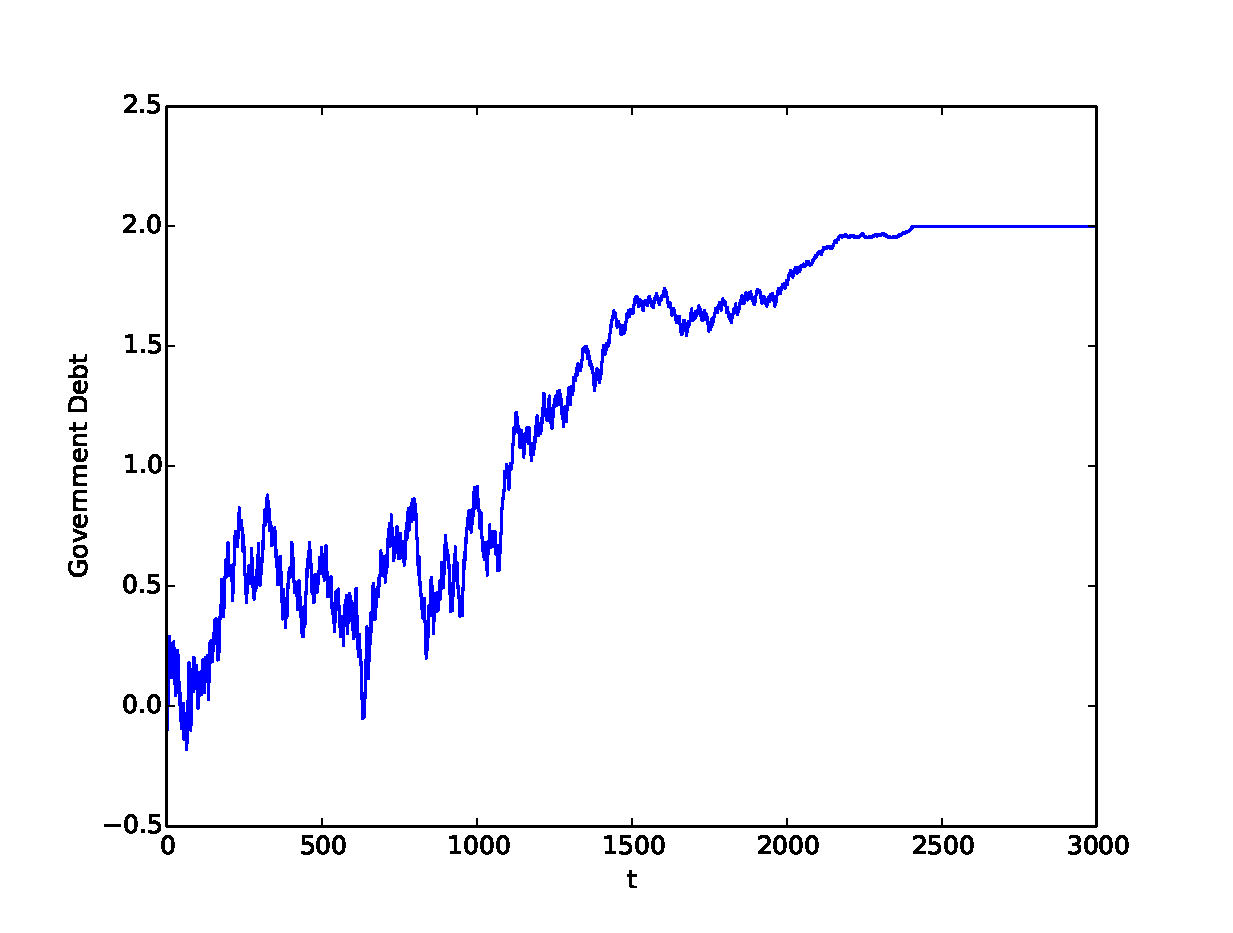
\includegraphics[width=4in]{Images/port1.eps}
	\end{center}
\end{frame}

\begin{frame}
	\frametitle{$p_1 < 1$}
	\begin{center}
	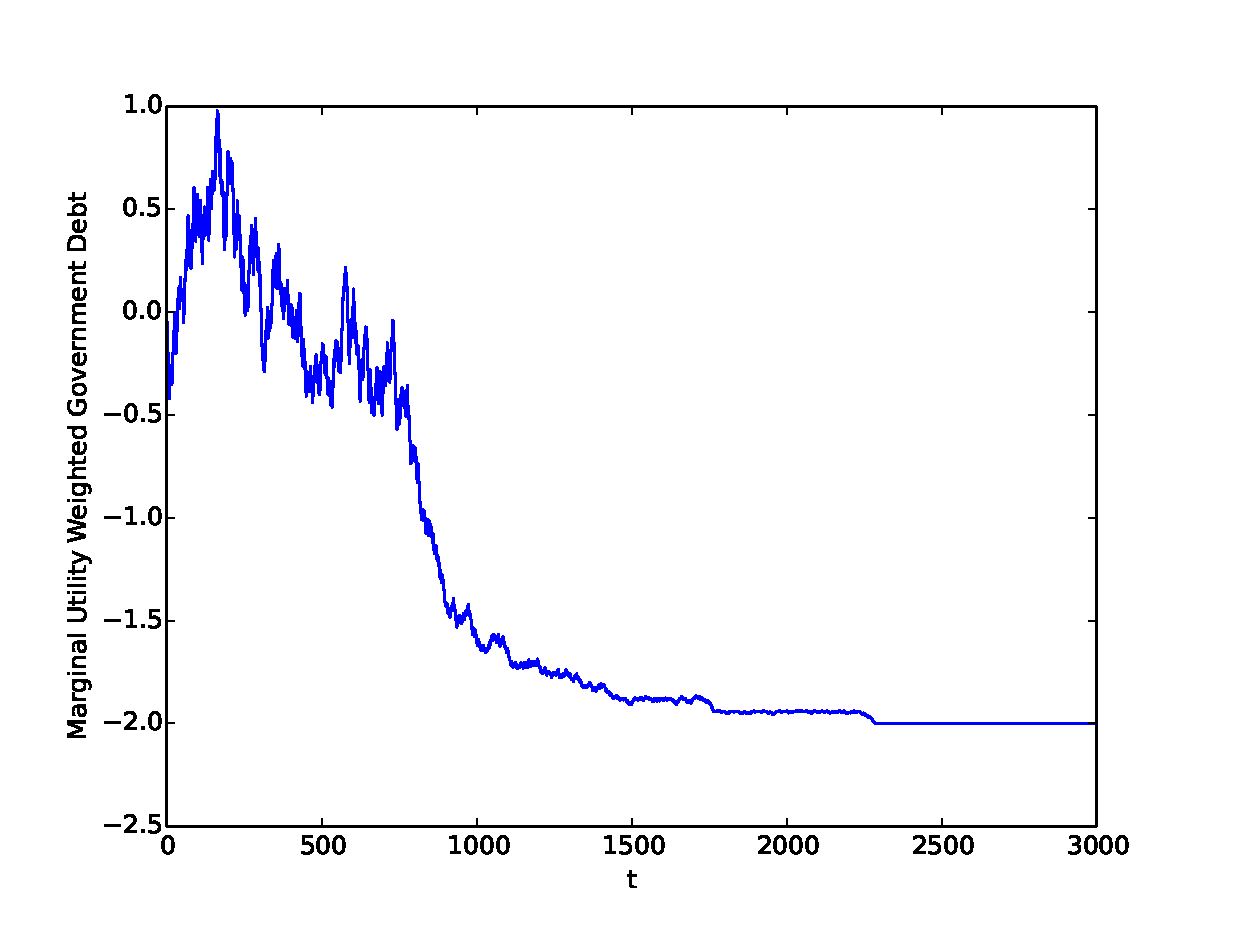
\includegraphics[width=4in]{Images/port2.eps}
	\end{center}
\end{frame}

\begin{frame}
	\frametitle{Intuition and Generalizations}
	\begin{itemize}
		\item The intuition we gain from our 2-state example is that, given exogenous payoff restrictions on government debt, there exist debt positions that allow the government to better smooth tax distortions across states.
		\item  Over time, the government adjusts it's debt position in order to best reallocate resources across states.
		\item  For more general aggregate state processes there no longer exists a complete markets steady state.
		\item  This requires us to develop computational tools to analyze the long-run dynamics.
		\item  We find that with more general processes there exist regions with low volatility, because the government's debt position is reallocating resources across states and in the long run the government debt converges to these regions.
	\end{itemize}
\end{frame}

\section{Risk Aversion}
\subsection{}

 \begin{frame}
 	\frametitle{Incomplete Markets Solution}
	\begin{itemize}
	\item By choosing a new state variable $x_{t-1} = b_{t-1} U_{c,t-1}$ the measurability constraints can be written as a period by period constraint
	\[
		\frac{x_{t-1} p_t U_{c,t}}{\beta \EE_{t-1} p_t U_{c,t}}  = U_{c,t}c_t+U_{l,t} l_t + x_t
	\]
	\item  This bares a striking resemblance to the period by period constraint for quasi-linear preferences
	\[
		\frac{b_{t-1} p_t}{\beta \EE_{t-1} p_t} = c_t + U_{l,t} l_t + b_t
	\]
	\item  In fact, when $p_t =1$ the $U_{c,t}$ terms in the risk averse budget constraint act as endogenous payoffs with higher returns in bad states of the world.
	\item  From our quasi linear results our intuition would then be that there exists a steady state in the 2-state i.i.d. environment where the government holds assets.
	\end{itemize}
\end{frame}

\begin{frame}
	\frametitle{Existence}
	Let $x_{fb}$ be the $x$ with which the government can institute first best from that period onwards.  Assume a CRRA utility specification $U(c,l) = \frac{c^{1-\sigma}}{1-\sigma} -\frac{ l^{1+\gamma}}{1+\gamma}$.  Finally, let  $c^{fb}$ and $l^{fb}$ be consumption and leisure under first best.  We have the following proposition
	\begin{proposition}  For a 2 state i.i.d. process let  $s_g$ and $s_b$ denoting the states with high and low consumption at first best.  If
	\[
		\frac{g(s_g)}{1-\frac{\beta\EE[(c^{fb})^{-\sigma}]}{c^{fb}(s_g)}} > \frac{g(s_b)}{1-\frac{\beta\EE[(c^{fb})^{-\sigma}]}{c^{fb}(s_b)}}
	\]  Then there exists a multiplier $\mu$ and complete markets solutions $c^\mu,l^\mu$ such that 
	\[
	\underline x<\frac{U_{c_\mu}(s)c_\mu(s) + U_{l_\mu}(s) l_\mu(s)}{\frac{U_{c_\mu}(s)}{\beta\EE[U_{c_\mu}]}-1} = x^* <0
	\]
	\end{proposition} 
\end{frame}


\begin{frame}
	\frametitle{Stability}
	The previous slide tells us that if the incomplete markets economy at some point reaches  $x^* < 0$ it will forever remain there, and the allocations will be identical to a time 1 complete markets allocation.  Moreover this point is before the planner can implement first best with transfers.  The question remains, will the economy converge to this point.
	\begin{proposition}  Let $\{c_t(s^t), l_t(s^t), x_t(s^{t-1})\}$ be the solution to the incomplete markets problem with $x_0 > x^*$.  Then  $x_t(s^{t-1})\rightarrow x^*$ as $t\rightarrow \infty$ with probability 1.
	\end{proposition}  Thus, if the economy starts with less assets then the complete markets steady state it will converge to this point with probability 1.
\end{frame}

\begin{frame}
	\frametitle{An Intuition}
	\begin{itemize}
		\item  What is the reason for the difference between the quasilinear and risk averse specification?
		\item  Under the quasilinear assumption with a risk free bond the interest rate is always $1/\beta$, while the risk averse problem has higher interest rates in period of high government expenditure.
		\item  Thus, while the government has greater expenses in high government expenditure states, the higher interest means that it has to invest less to cover future government expenditures.
		\item  Once the government has accumulated enough assets, it is actually better off in periods of high government expenditure than low government expenditures (since it's claims to consumption of worth more).
		\item  By holding assets the government is able to reallocate resources across states, something it was not able to do in the quasilinear case.
	\end{itemize}
\end{frame}

\begin{frame}
	\frametitle{2 State i.i.d. process with Risk Aversion}
	\begin{center}
	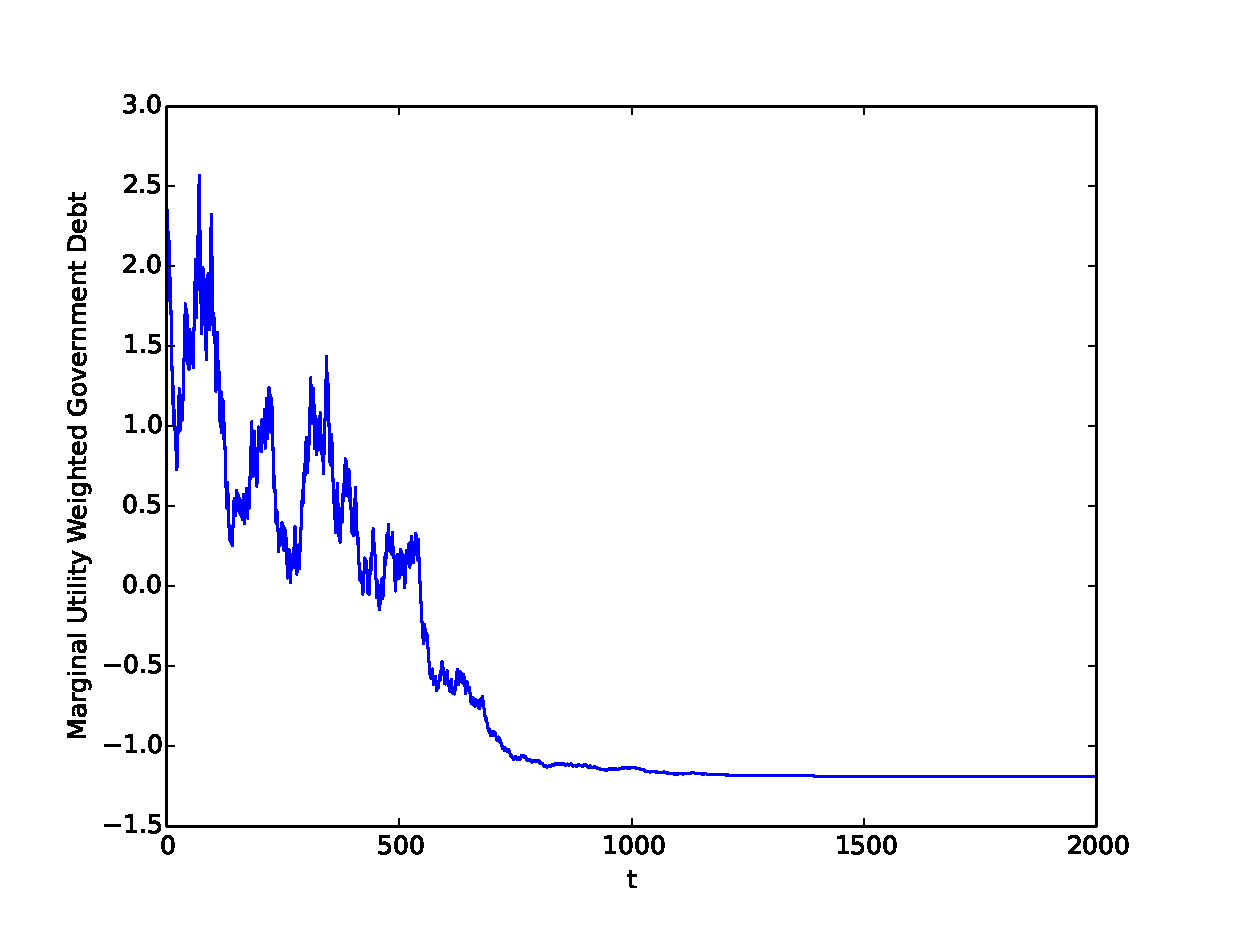
\includegraphics[width=4in]{Images/2stateiid.eps}
	\end{center}
\end{frame}
  
\section{Numerical Results}
\subsection{}

 \begin{frame}
	\frametitle{A Recursive Approach: Time $t\geq 1$ }
	The ability to write the period by period budget constraint as 
	\[
		\frac{x_{t-1} p_t U_{c,t}}{\beta \EE_{t-1} p_t U_{c,t}}  = U_{c,t}c_t+U_{l,t} l_t + x_t
	\]Allows us to write the planner's problem recursively with a single state variable.  The time $t\geq 1$  Bellman equation is then
	\[
		V(x,s\_) = \max_{c(s),l(s),x'(s)} \sum_s \pi(s,s\_)\left(U(c(s),l(s)) + \beta V(x'(s),s)\right)
	\]subject to $x'(s)\in [\underline x,\overline x]$
	\begin{align*}
		\frac{x p(s) U_c(s)}{\beta\EE pUc} \leq U_c(s)c(s)+U_l(s)l(s) + x'(s)\\
		c(s) + g(s) = \theta(s)l(s)
	\end{align*}  Note the inequality allows for positive transfers.  Moreover, $x$ is a time consistent state variable.
 \end{frame}

\begin{frame}
	\frametitle{A Recursive Approach: Time 0}
	Given the initial debt level $b_0$, state $s_0$,  and the continuation value function $V(x,s\_)$ the planner's problem is then to solve the following
	\[
		\max_{c,l,x'} U(c,l) +\beta V(x',s0)
	\]subject to the time zero implementability constraint
	\[
		U_{c}(c,l)c + U_l(c,l) l + x' \geq U_c(c,l) b_0
	\]and the resource constraint
	\[
		c+ g(s_0) = \theta l
	\]and
	\[
		x' \in [\underline x,\overline x]
	\]
\end{frame}

\begin{frame}
	\frametitle{$S>2$ states}
	\begin{center}
	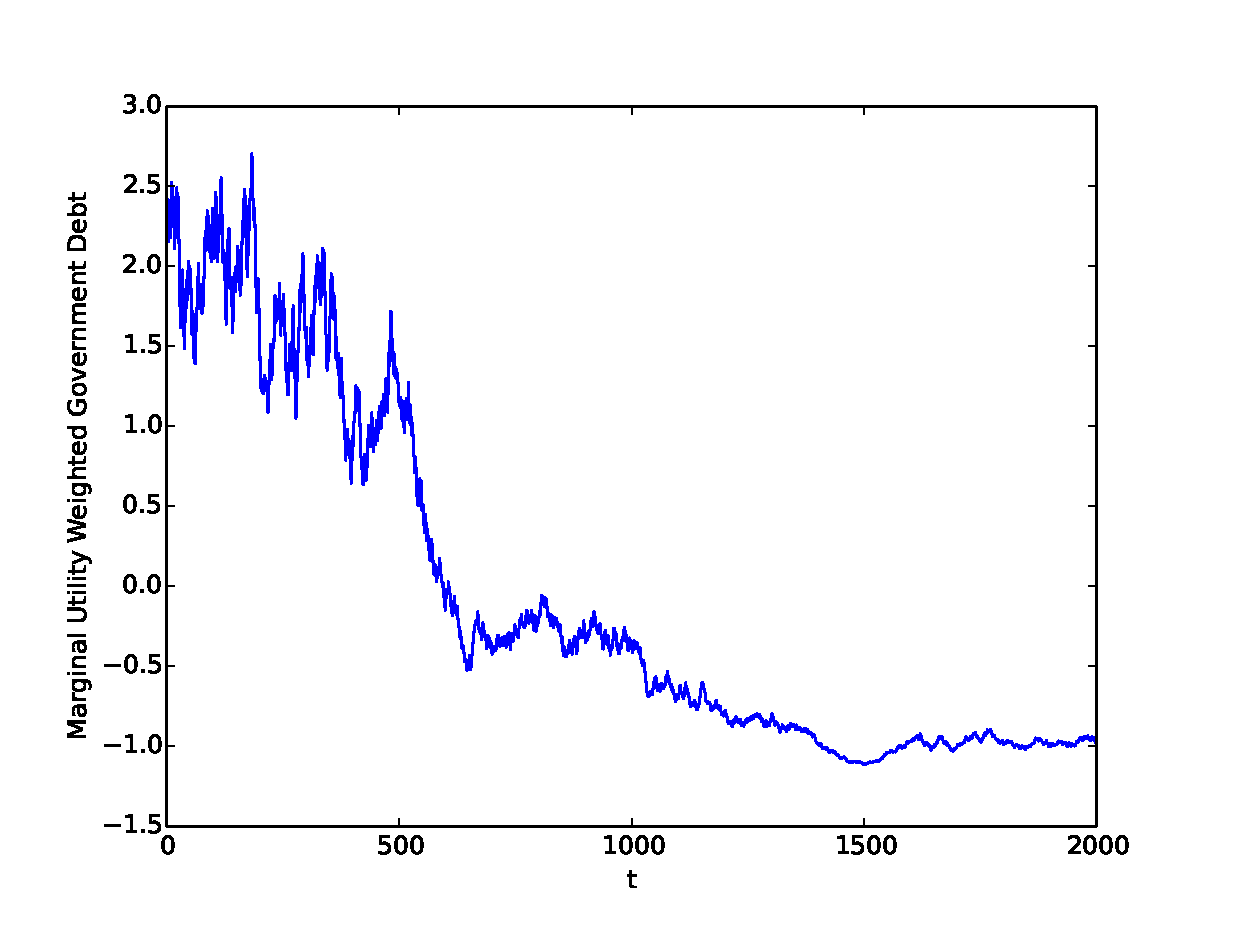
\includegraphics[width=4in]{Images/5stateiid.eps}
	\end{center}
\end{frame}


\begin{frame}
	\frametitle{AMSS Calibration}
	\begin{center}
	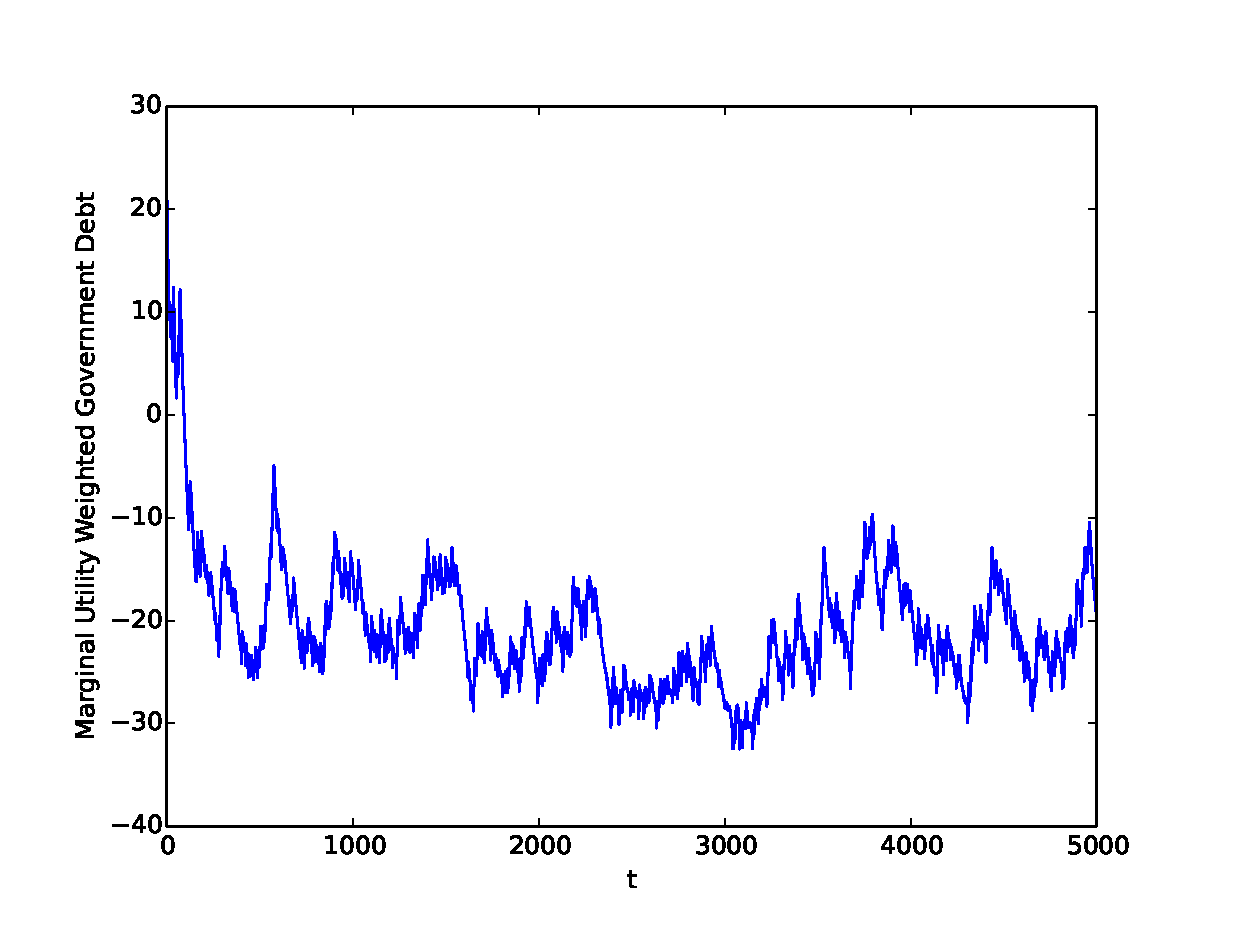
\includegraphics[width=4in]{Images/AMSS.eps}
	\end{center}
\end{frame}


 \begin{frame}
  \frametitle{The Role of Transfers}
	\begin{itemize}
		\item  Most of our theoretical results were derived under the assumption that the government did not have access to lump sum transfers.
		\item  Even with lump sum transfers the cases where the steady state exists and is stable, if the initial debt of the government starts out above the steady state level the economy will converge with probability 1 to the steady state.
		\item  If a steady state does not exist we need to use numerical methods to simulate long run paths of the system.
		\item  We find that the existence of transfers plays little role in the optimal allocations, even in the few calibrations where the AMSS results conclude that the economy will converge to first best with probability 1.
		\item  The intuition that the government we use it's asset position to smooth taxation distortions carries over even when the government has access to lump sum transfers.
	\end{itemize}
 \end{frame}

 \begin{frame}
	\frametitle{AMSS calibration with and without transfers}
	\begin{center}
	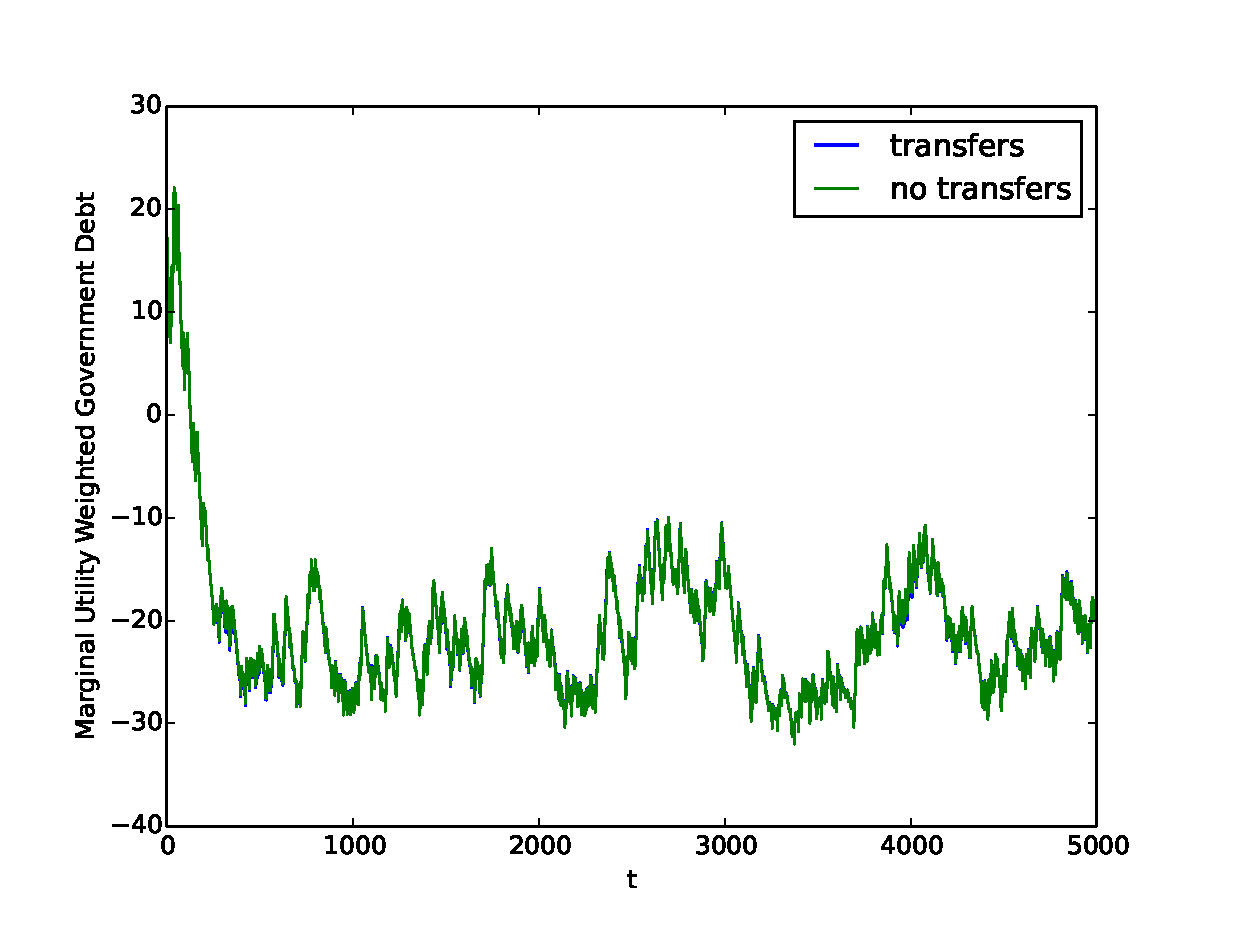
\includegraphics[width=4in]{Images/transfer_example1.eps}
	\end{center}
\end{frame}

\begin{frame}
	\frametitle{Quasilinear Preferences and Risk Free Bond  with and without Transfers}
	\begin{center}
	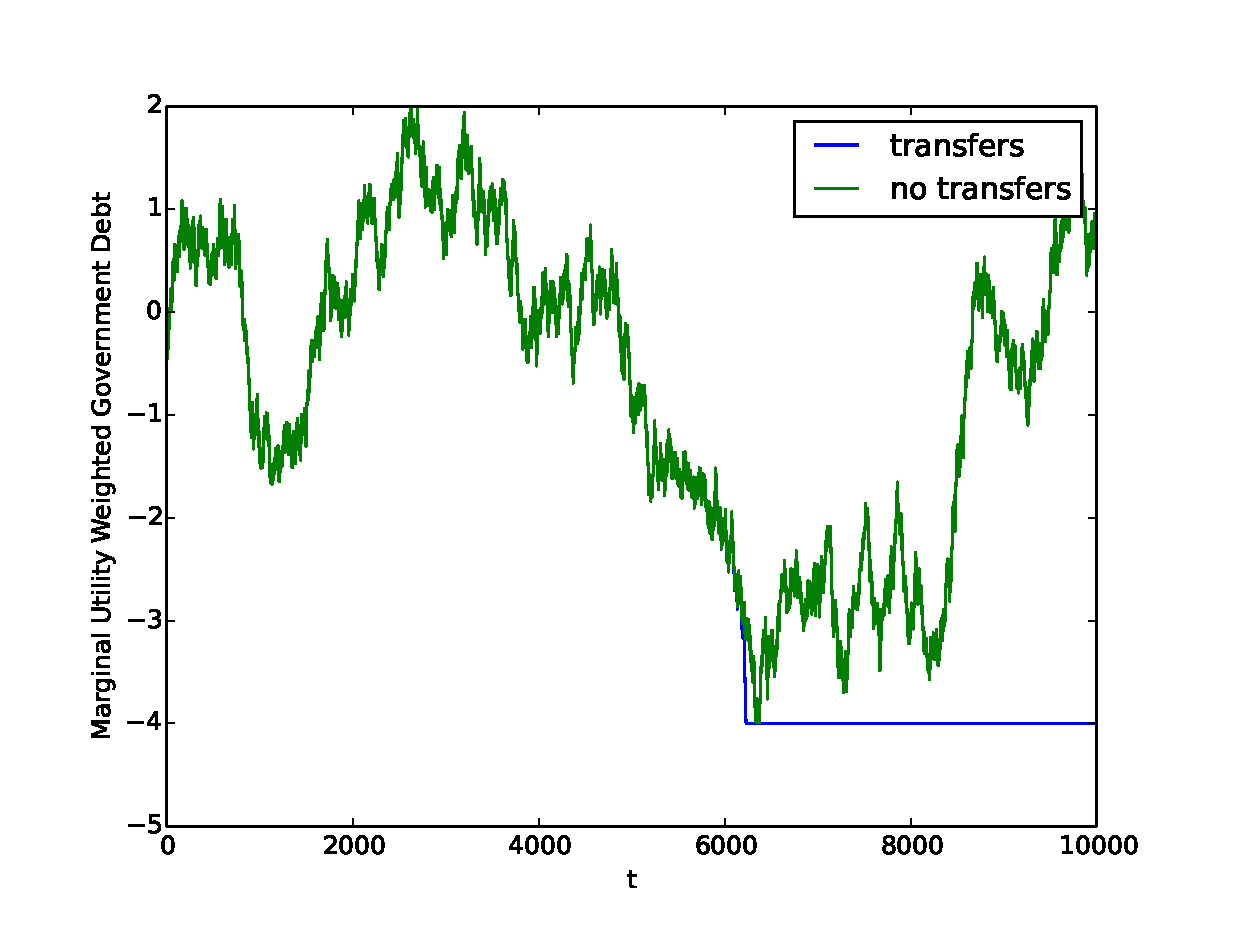
\includegraphics[width=4in]{Images/transfer_example2.eps}
	\end{center}
\end{frame}

 \begin{frame}
  \frametitle{Conclusion}
\begin{itemize}
	\item We find that the nature of market incompleteness has drastic implications for the long run debt position of the government in an optimal planning problem.
	\item If the payoff structure of government assets has greater returns in good states of the world then bad, then the government will accumulate debt in the long run.
	\item  With risk aversion, the payoff structure of the time-consistent savings variable is what determines the long run debt position of the government.
	\item  Transfers play little role in determining the evolution of the system.  Rather the key motivating force is using debt position to reallocate recourses across states.
	\item  \textbf{Future Research}:  How does the type of market incompleteness effect long run wealth distributions with heterogeneous agents
\end{itemize}
 \end{frame}

 \end{document}
 